\documentclass[a4paper,12pt]{article}

\usepackage{amsmath}
\usepackage{amsfonts}
\usepackage{array}
\usepackage{color}
\usepackage{enumitem}
\usepackage{graphicx}
\usepackage{indentfirst}
\usepackage{listings}
\usepackage{makecell}
\usepackage{tabularx}
\usepackage[T2A]{fontenc}
\usepackage[russian]{babel}
\usepackage[left=3cm, right=1cm, top=2cm, bottom=2cm]{geometry}

\definecolor{bg}{rgb}{1.0,1.0,0.6}
\definecolor{text}{rgb}{0.0,0.0,0.0}
\lstdefinestyle{mystyle}{
    backgroundcolor=\color{bg},   
    commentstyle=\color{text},
    keywordstyle=\color{text},
    numberstyle=\tiny\color{text},
    stringstyle=\color{text},
    basicstyle=\ttfamily\footnotesize,
    breakatwhitespace=false,         
    breaklines=true,                 
    captionpos=b,                    
    keepspaces=true,                 
    numbers=left,                    
    numbersep=5pt,                  
    showspaces=false,                
    showstringspaces=false,
    showtabs=false,                  
    tabsize=2
}

\lstset{style=mystyle}

\begin{document}

\begin{center}
    {\small Федеральное государственное автономное образовательное учреждение высшего образования \\
<<Национальный исследовательский ядерный университет ``МИФИ''>> \\
    Кафедра №12 <<Компьютерные системы и технологии>>}
\end{center}

\vspace*{\fill}
\begin{center}
    {\Large \textbf{ЛАБОРАТОРНАЯ РАБОТА №2}} \\
    \bigskip
    По дисциплине <<Цифровая схемотехника>>\\
    \bigskip
    \textbf{Тема:} Синтез комбинационных схем\\
    \bigskip
    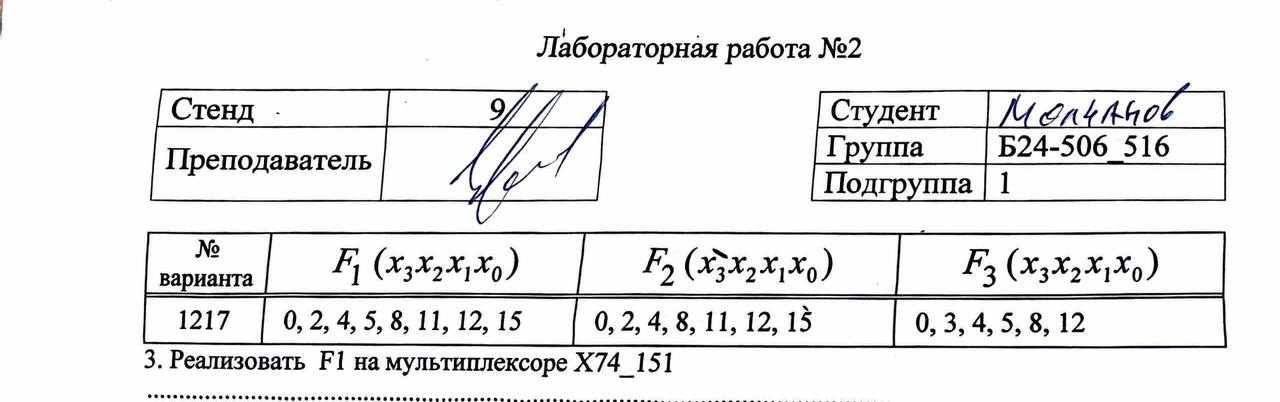
\includegraphics[width=1\textwidth]{pic2.jpg}\\
\end{center}
\vspace*{\fill}

\begin{flushright}
    \textbf{Выполнил студент:}\\
    Молчанов Степан Андреевич\\
    \textbf{Группа:} Б24-516\\
    \textbf{Логин:} B24\_516\_09\\
    \textbf{Пароль:} AD0sW17p
\end{flushright}

\begin{center}
    Москва\\
    2026
\end{center}

\newpage

\section*{Цель работы}
Изучить методы синтеза комбинационных схем на логических элементах; 
получить навыки проектирования комбинационных схем на VHDL; 
овладеть инструментальными средствами проектирования схем на ПЛИС; 
приобрести опыт экспериментального исследования синтезируемых схем.

\section*{Ход работы}
Таблица 2.1. Таблица истинности системы логических функций
\begin{table}[h]
    \centering

    \setlength{\arrayrulewidth}{0.4pt}

    \newcommand{\thickhline}{%
        \noalign{\hrule height 1.2pt}
    }

    \begin{tabular}{
        !{\vrule width 1.2pt}
        c
        !{\vrule width 1.2pt}
        c|c|c|c
        !{\vrule width 1.2pt}
        c|c|c
        !{\vrule width 1.2pt}
    }

        % Верхняя граница
        \thickhline

        % Заголовок
        № & $x_3$ & $x_2$ & $x_1$ & $x_0$ & $F_1$ & $F_2$ & $F_3$ \\

        % Граница под заголовком
        \thickhline

        % Данные
        0  & 0 & 0 & 0 & 0 & 1 & 1 & 1 \\
        \hline
        1  & 0 & 0 & 0 & 1 & 0 & 0 & 0 \\
        \hline
        2  & 0 & 0 & 1 & 0 & 1 & 1 & 0 \\
        \hline
        3  & 0 & 0 & 1 & 1 & 0 & 0 & 1 \\
        \hline
        4  & 0 & 1 & 0 & 0 & 1 & 1 & 1 \\
        \hline
        5  & 0 & 1 & 0 & 1 & 1 & 0 & 1 \\
        \hline
        6  & 0 & 1 & 1 & 0 & 0 & 0 & 0 \\
        \hline
        7  & 0 & 1 & 1 & 1 & 0 & 0 & 0 \\
        \hline
        8  & 1 & 0 & 0 & 0 & 1 & 1 & 1 \\
        \hline
        9  & 1 & 0 & 0 & 1 & 0 & 0 & 0 \\
        \hline
        10 & 1 & 0 & 1 & 0 & 0 & 0 & 0 \\
        \hline
        11 & 1 & 0 & 1 & 1 & 1 & 1 & 0 \\
        \hline
        12 & 1 & 1 & 0 & 0 & 1 & 1 & 1 \\
        \hline
        13 & 1 & 1 & 0 & 1 & 0 & 0 & 0 \\
        \hline
        14 & 1 & 1 & 1 & 0 & 0 & 0 & 0 \\
        \hline
        15 & 1 & 1 & 1 & 1 & 1 & 1 & 0 \\

        % Нижняя граница
        \thickhline

    \end{tabular}
\end{table}

\begin{center}
    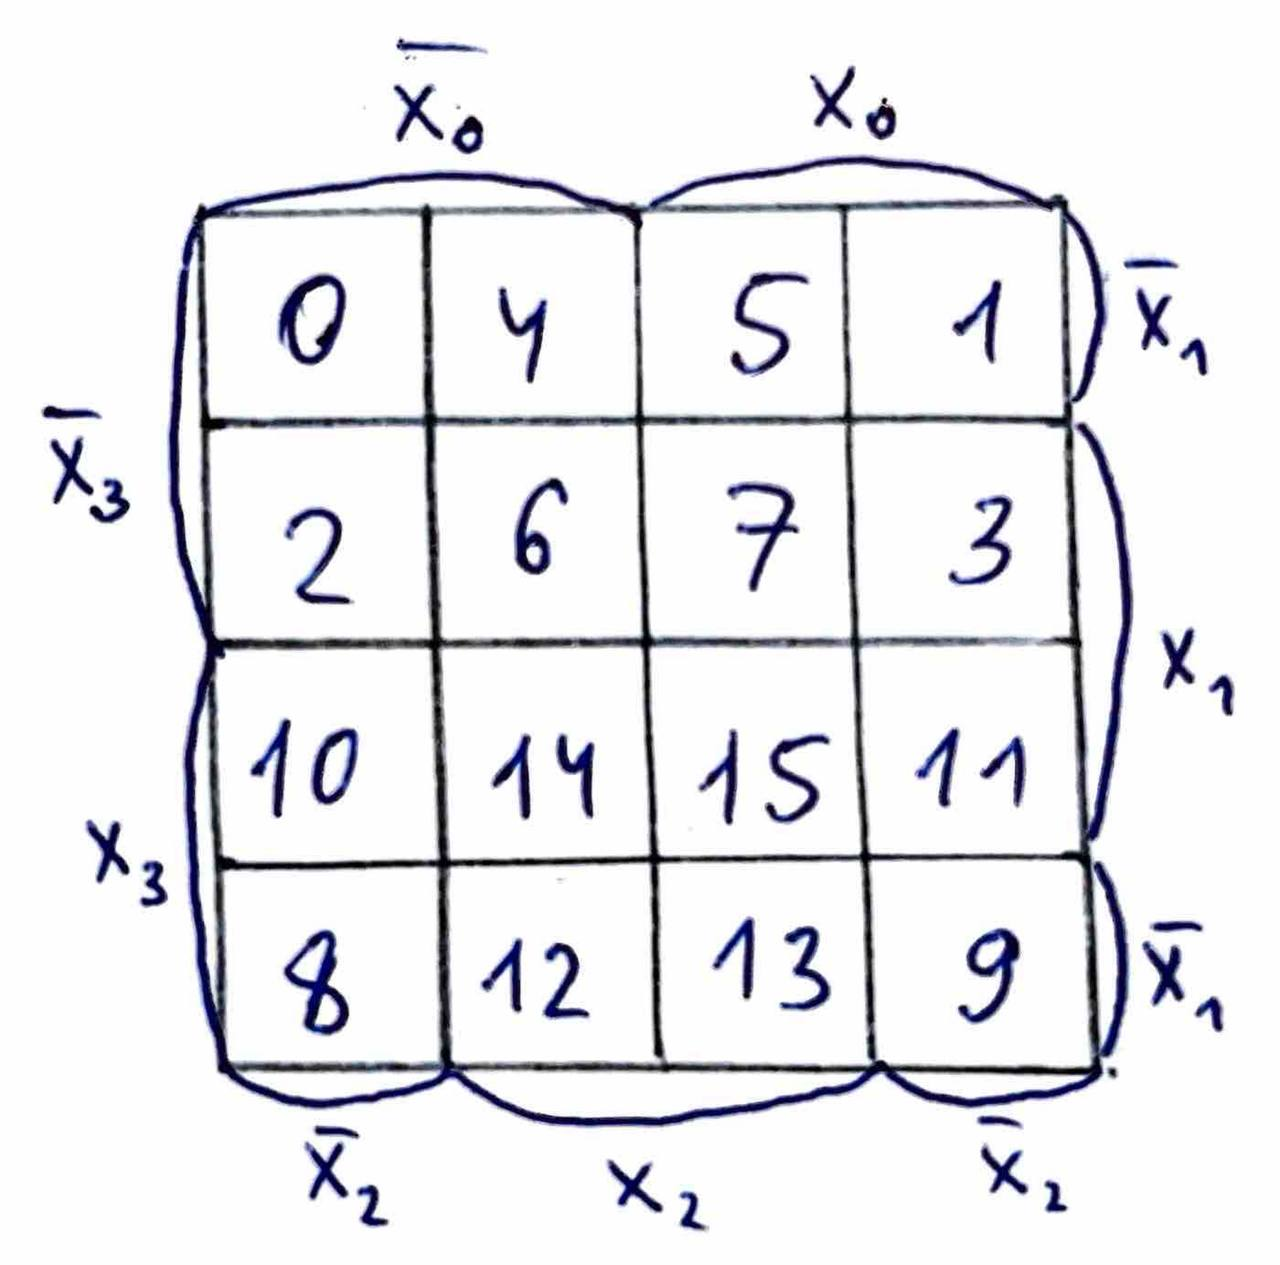
\includegraphics[width=0.5\textwidth]{pic3.jpg} \\
    {\small Рис. 2.1. Эталонная диаграмма Вейча для функций четырёх аргументов}
\end{center}

\begin{center}
    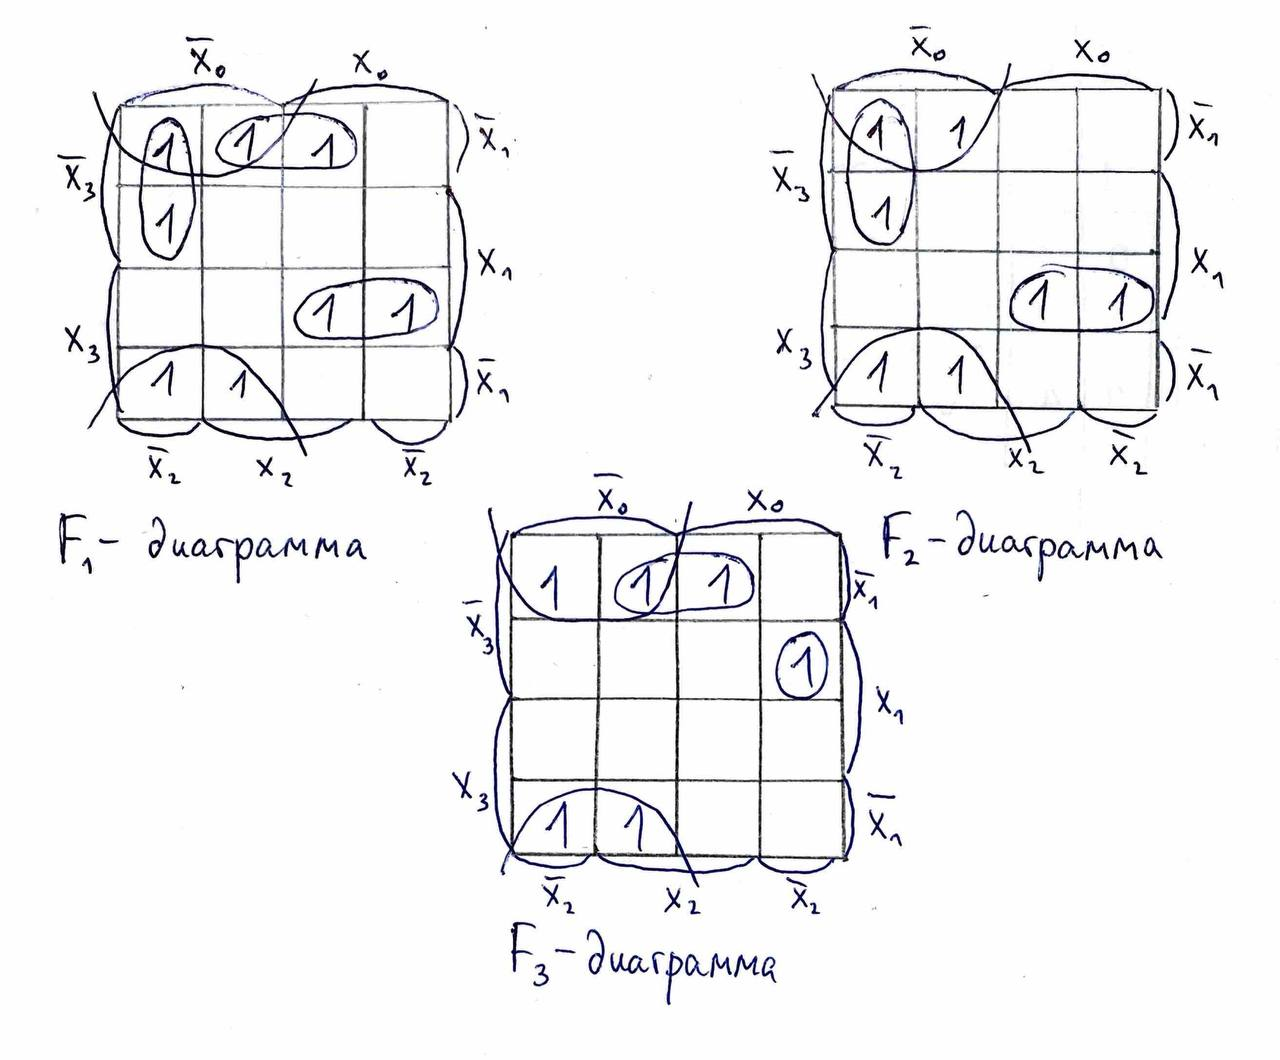
\includegraphics[width=0.7\textwidth]{pic4.jpg} \\
    {\small Рис. 2.2. Диаграммы Вейча трёх функций}
\end{center}

Простые импликанты для функций $F_1$, $F_2$ и $F_3$:

\begin{equation}
    \tag{2.1}
    \left.
    \begin{aligned}
        &F_1 = \bar{x_1}\bar{x_0}\ \lor\ x_3x_1x_0\ \lor\ \bar{x_3}\bar{x_2}\bar{x_0}\ \lor\ \bar{x_3}x_2\bar{x_1} \\
        &F_2 = \bar{x_1}\bar{x_0}\ \lor\ x_3x_1x_0\ \lor\ \bar{x_3}\bar{x_2}\bar{x_0} \\
        &F_3 = \bar{x_1}\bar{x_0}\ \lor\ \bar{x_3}x_2\bar{x_1}\ \lor\ \bar{x_3}\bar{x_2}x_1x_0
    \end{aligned}
    \right\}
\end{equation}

\begin{center}
    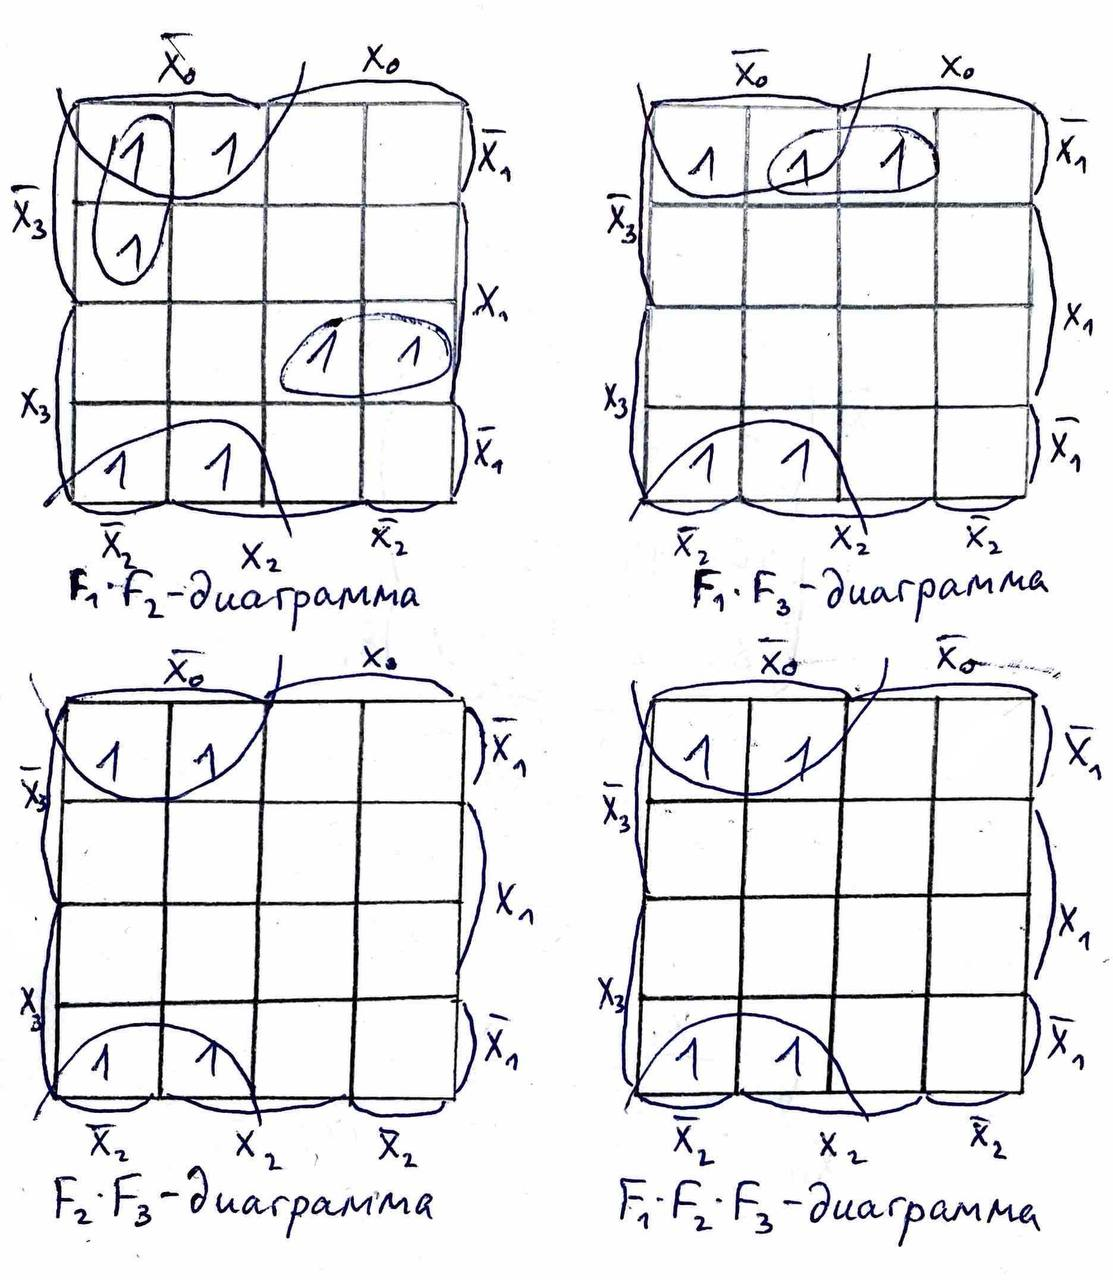
\includegraphics[width=0.5\textwidth]{pic5.jpg} \\
    {\small Рис. 2.3. Диаграммы Вейча логических произведений трёх функций}
\end{center}

По полученным диаграммам найдём простые импликанты данных функций:
\begin{equation}
    \tag{2.2}
    \left.
    \begin{aligned}
        &F_1 \cdot F_2\ =\ \bar{x_1}\bar{x_0}\ \lor\ x_3x_1x_0\ \lor\ \bar{x_3}\bar{x_2}\bar{x_0} \\
        &F_2 \cdot F_3\ =\ \bar{x_1}\bar{x_0}\ \lor\ \bar{x_3}x_2\bar{x_1} \\
        &F_2 \cdot F_3\ =\ \bar{x_1}\bar{x_0} \\
        &F_1 \cdot F_2 \cdot F_3\ =\ \bar{x_1}\bar{x_0}
    \end{aligned}
    \right\}
\end{equation}

\begin{flushright}
    Таблица 2.2
\end{flushright}

\begin{center}
    \textbf{Импликантная матрица системы логических функций}
    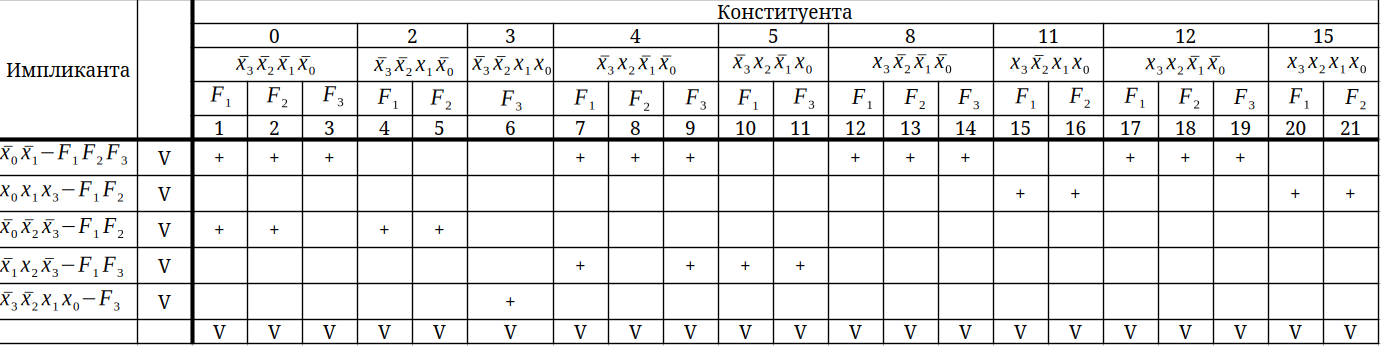
\includegraphics[width=1\textwidth]{pic6.png}
\end{center}

Выбирая для каждой функции минимально возможное количество отмеченных импликант, получаем искомую минимальную совокупность переключаемых функций:
\begin{equation}
    \tag{2.3}
    \left.
    \begin{aligned}
        &F_1 = \bar{x_1}\bar{x_0}\ \lor\ x_3x_1x_0\ \lor\ \bar{x_3}\bar{x_2}\bar{x_0}\ \lor\ \bar{x_3}x_2\bar{x_1} \\
        &F_2 = \bar{x_1}\bar{x_0}\ \lor\ x_3x_1x_0\ \lor\ \bar{x_3}\bar{x_2}\bar{x_0}\ \\
        &F_3 = \bar{x_1}\bar{x_0}\ \lor\ \bar{x_3}x_2\bar{x_1}\ \lor\ \bar{x_3}\bar{x_2}x_1x_0
    \end{aligned}
    \right\}
\end{equation}

Переведём данные логические функции в базис И-НЕ (штрих Шеффера):
\begin{equation}
    \tag{2.4}
    \left.
    \begin{aligned}
        &F_1 = (\bar{x_1}\ |\ \bar{x_0})\ |\ (x_3\ |\ x_1\ |\ x_0)\ |\ (\bar{x_3}\ |\ \bar{x_2}\ |\ \bar{x_0})\ |\ (\bar{x_3}\ |\ x_2\ |\ \bar{x_1})\\
        &F_2 = (\bar{x_1}\ |\ \bar{x_0})\ |\ (x_3\ |\ x_1\ |\ x_0)\ |\ (\bar{x_3}\ |\ \bar{x_2}\ |\ \bar{x_0})\\
        &F_3 = (\bar{x_1}\ |\ \bar{x_0})\ |\ (\bar{x_3}\ |\ x_2\ |\ \bar{x_1})\ |\ (\bar{x_3}\ |\ \bar{x_2}\ |\ x_1\ |\ x_0)
    \end{aligned}
    \right\}
\end{equation}

\begin{center}
    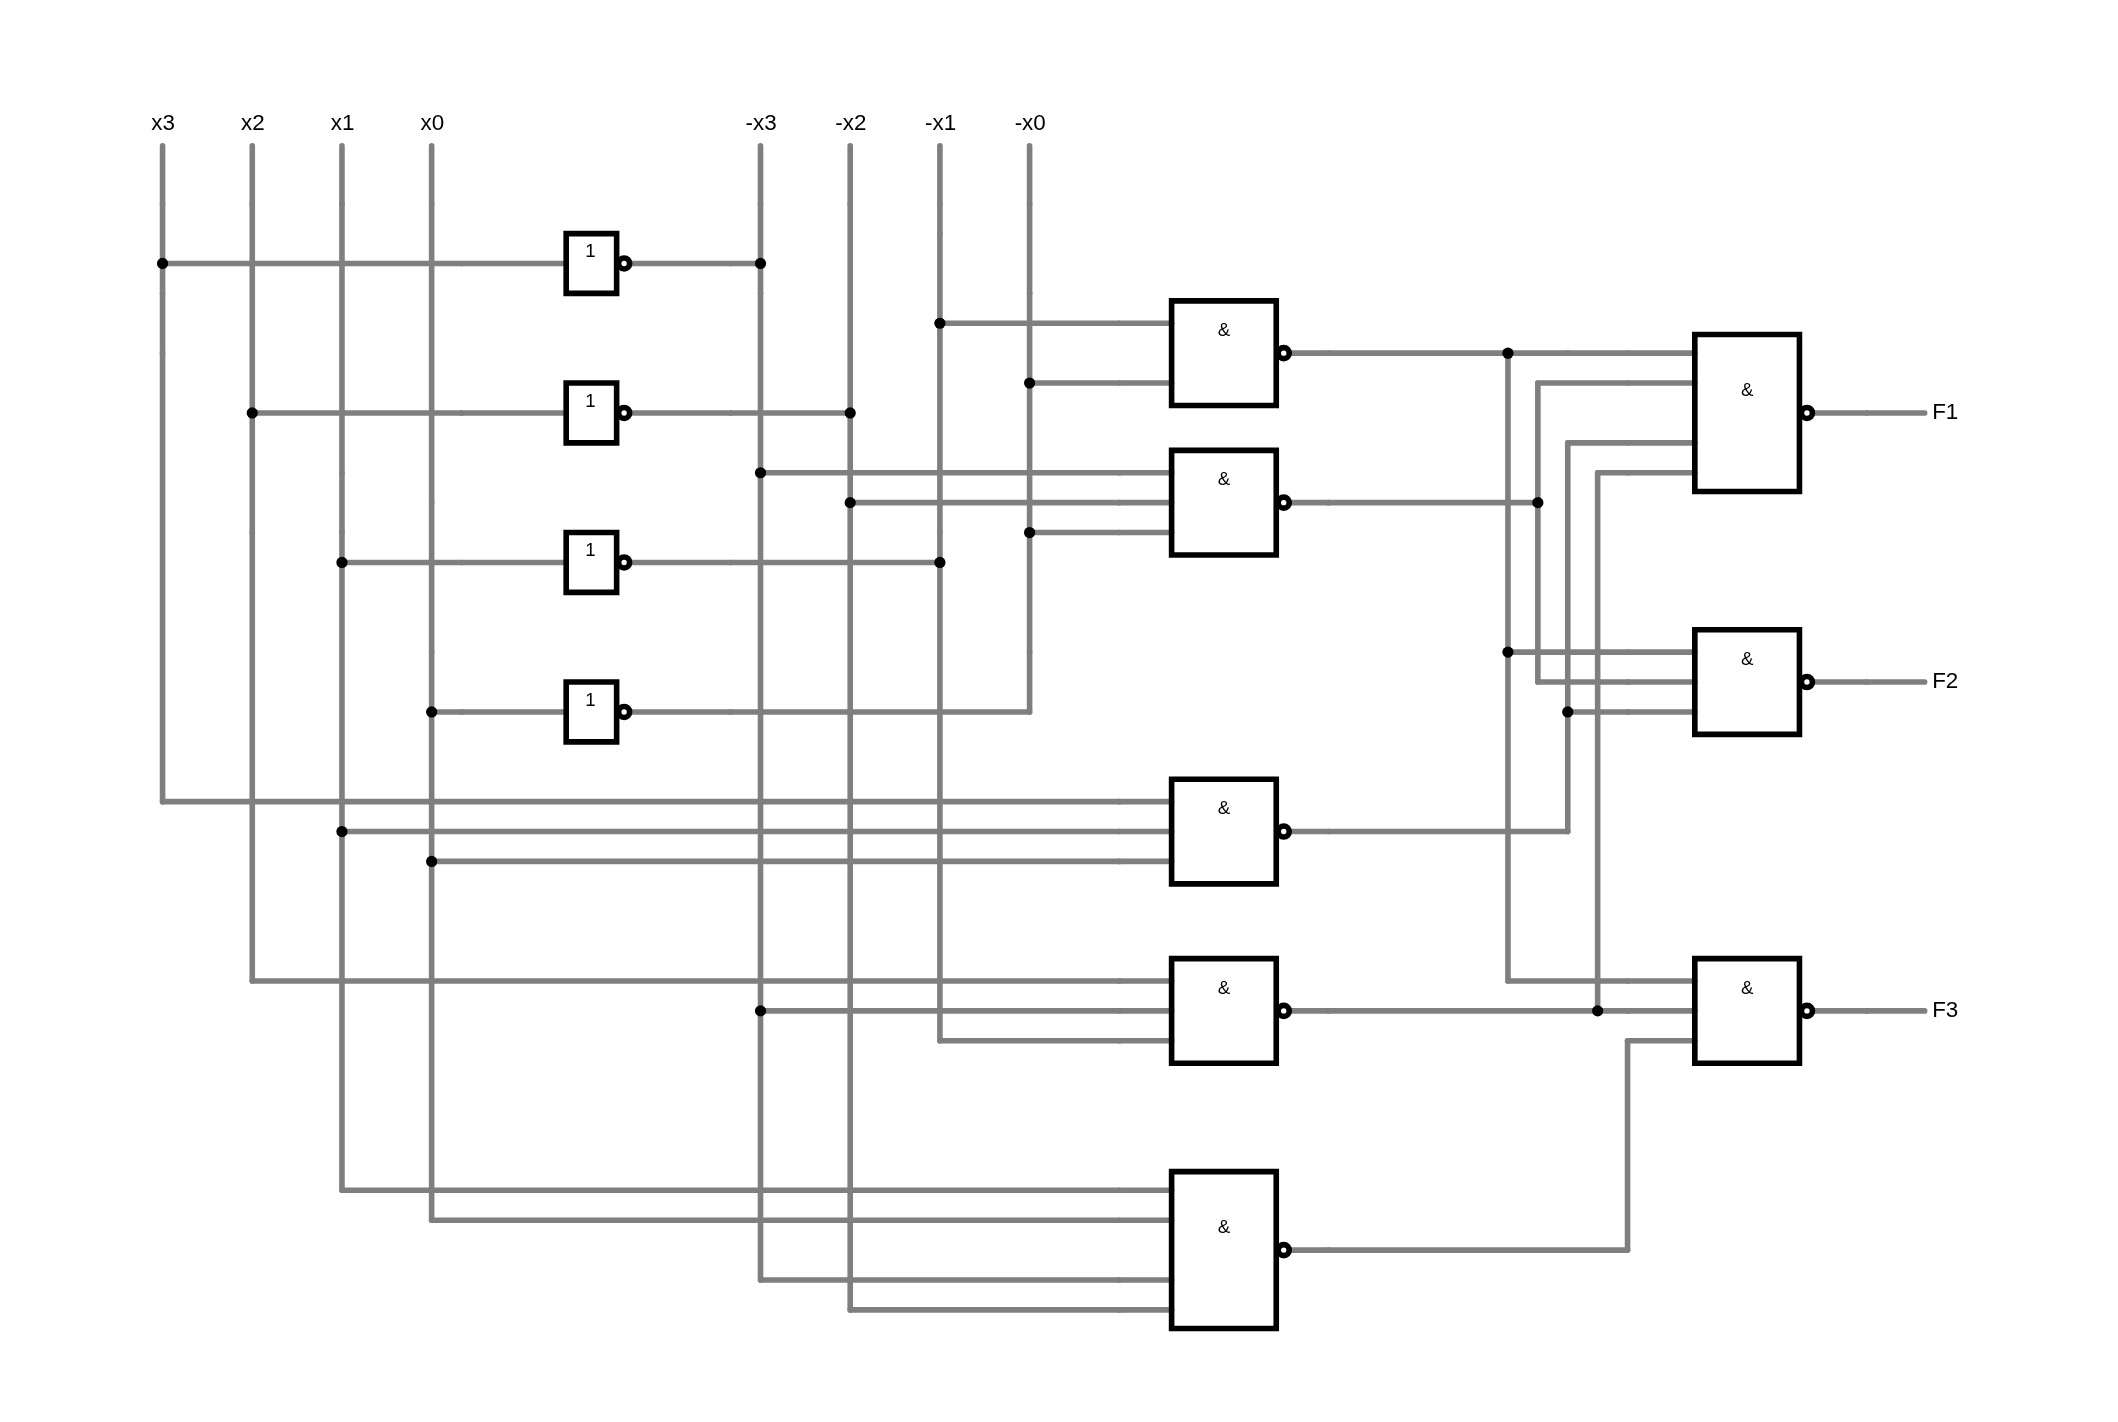
\includegraphics[width=1\textwidth]{pic7.png}\\
    {\small Рис. 2.4. Реализация многовыходной комбинационной схемы}
\end{center}

\newpage

\begin{center}
    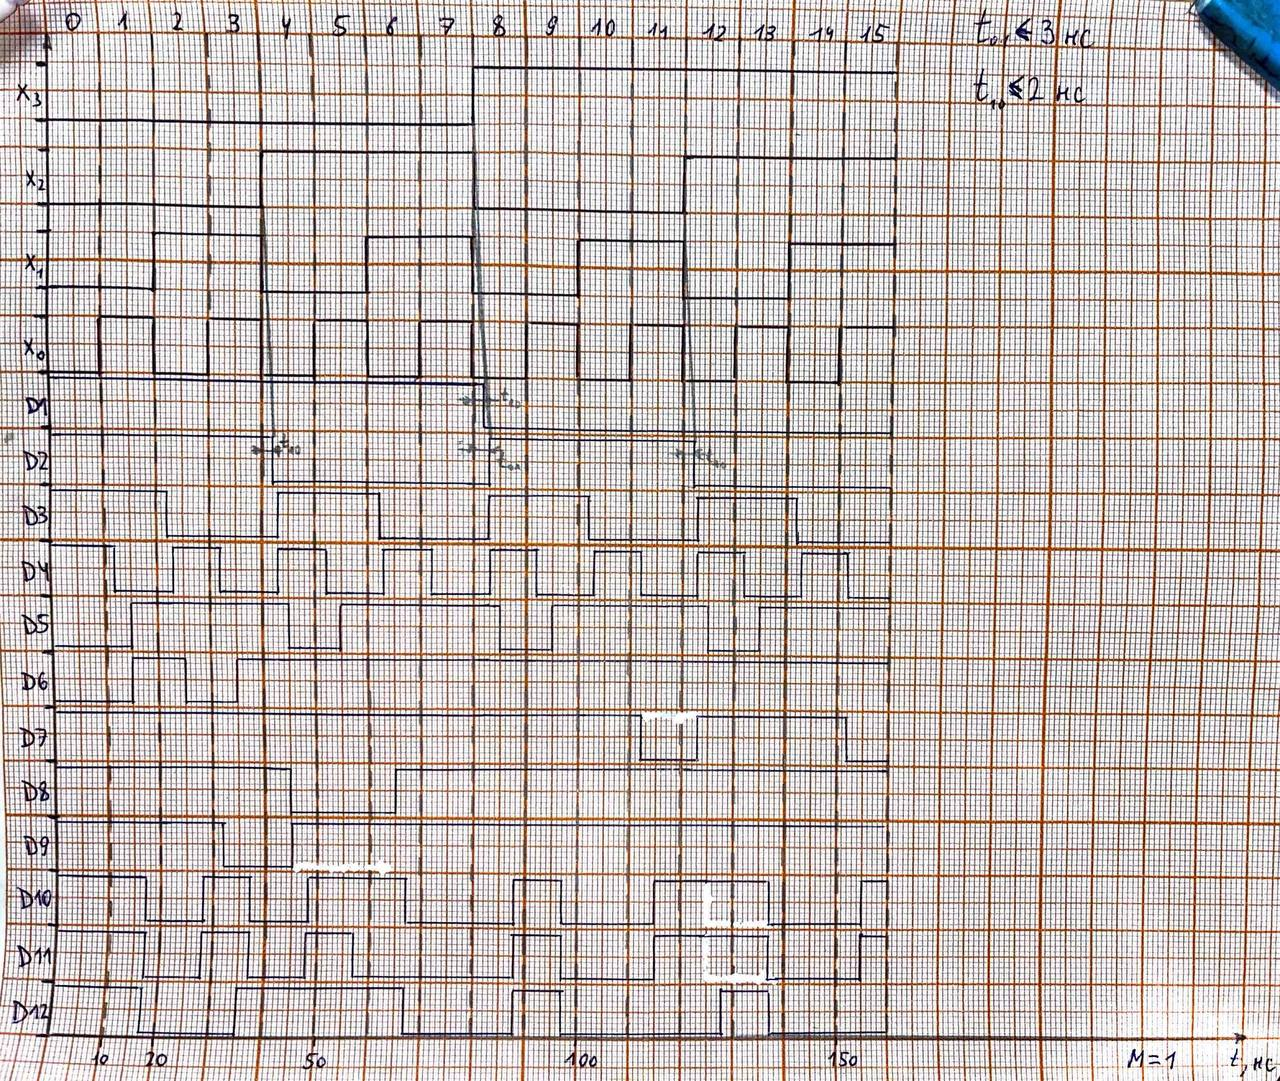
\includegraphics[width=0.9\textwidth]{pic8.jpg}\\
    {\small Рис. 2.5. Временная диаграмма комбинационной схемы (теоретический расчёт)}
\end{center}

\begin{center}
    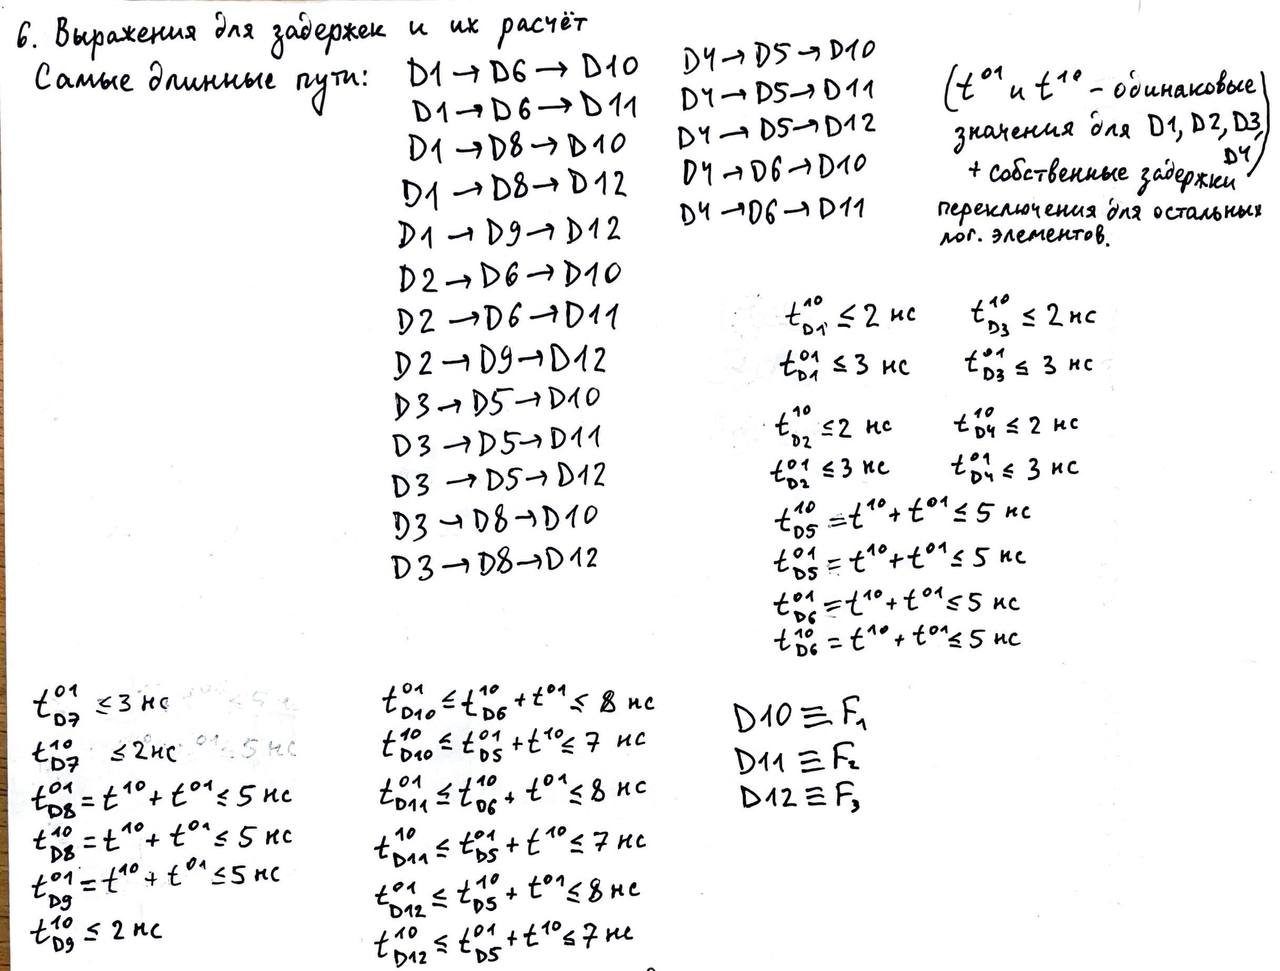
\includegraphics[width=0.7\textwidth]{pic9.jpg}\\
    {\small Рис. 2.6. Расчёт задержек многовыходной комбинационной схемы}
\end{center}

\newpage

\begin{center}
    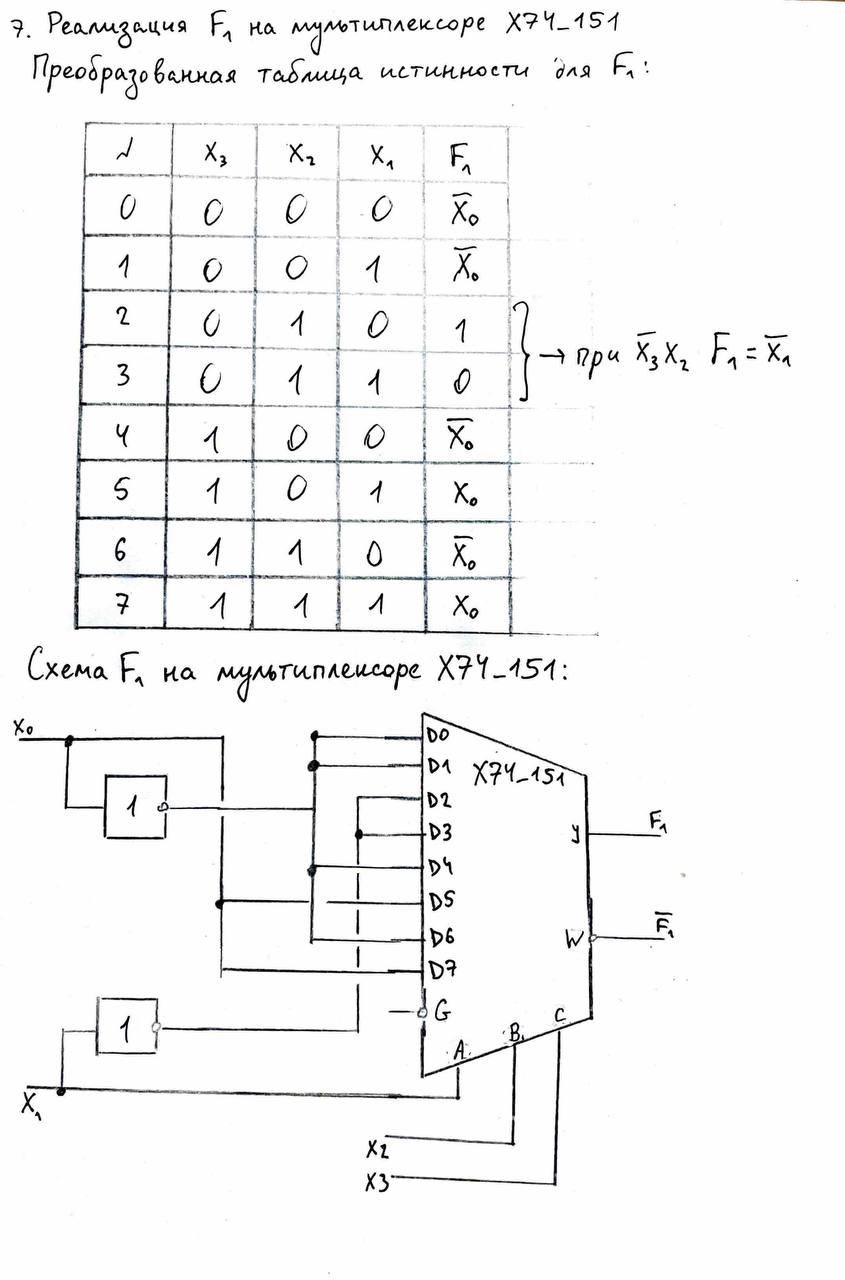
\includegraphics[width=0.9\textwidth]{pic10.jpg}\\
    {\small Рис. 2.7. Реализация $F1$ на мультиплексоре $X74\_151$}
\end{center}

\newpage

\begin{lstlisting}[language=VHDL, caption=Описание комбинационной схемы на языке VHDL.]
entity KS_VHDL is
    port (
        X0, X1, X2, X3: in BIT;
        F1: out BIT;
        F2: out BIT;
        F3: out BIT
    );
end KS_VHDL;

architecture KS_VHDL_arch of KS_VHDL is
    begin
        F1 <= (not X1 and not X0) or (X3 and X1 and X0) or 
    (not X3 and not X2 and not X0) or (not X3 and X2 and not X1);
        F2 <= (not X1 and not X0) or (X3 and X1 and X0) or 
    (not X3 and not X2 and not X0);
        F3 <= (not X1 and not X0) or (not X3 and X2 and not X1) or 
    (not X3 and not X2 and X1 and X0);
end KS_VHDL_arch;

\end{lstlisting}

\begin{center}
    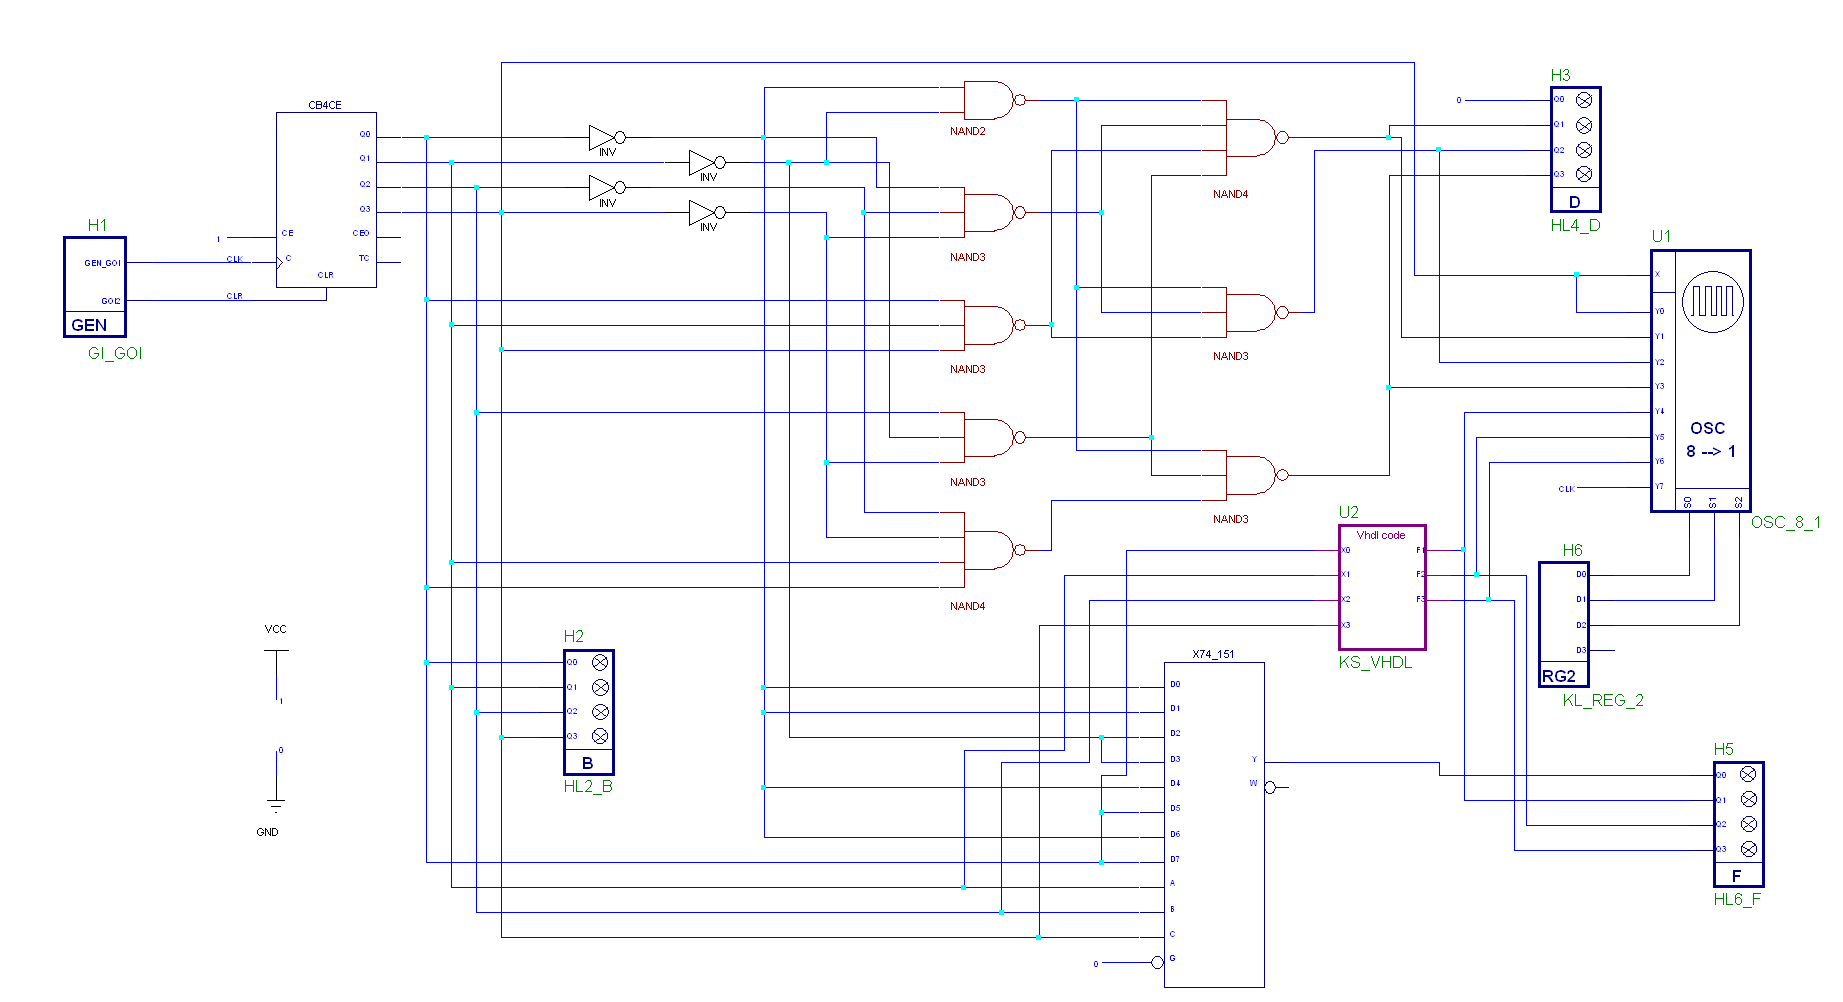
\includegraphics[width=1\textwidth]{pic1337.png}\\
    {\small Рис. 2.8. Схема, подготовленная для размещения на кристалле}
\end{center}

\end{document}
